%--------------------------------------------------------------------%
%
% Berkas utama templat LaTeX.
%
% author Petra Barus, Peb Ruswono Aryan
%
%--------------------------------------------------------------------%
%
% Berkas ini berisi struktur utama dokumen LaTeX yang akan dibuat.
%
%--------------------------------------------------------------------%

\documentclass[12pt, a4paper, onecolumn, oneside, final]{report}

%-------------------------------------------------------------------%
%
% Konfigurasi dokumen LaTeX untuk laporan tesis IF ITB
%
% @author Petra Novandi
%
%-------------------------------------------------------------------%
%
% Berkas asli berasal dari Steven Lolong
%
%-------------------------------------------------------------------%

% Ukuran kertas
\special{papersize=210mm,297mm}

% Setting margin
\usepackage[top=3cm,bottom=2.5cm,left=4cm,right=2.5cm]{geometry}

\usepackage{mathptmx}
\usepackage{amsmath}
\usepackage{float}

% Judul bahasa Indonesia
\usepackage[bahasa]{babel}

% section kode
\usepackage{listings}
\lstdefinestyle{customc}{
  belowcaptionskip=1\baselineskip,
  breaklines=true,
  frame=single,
  xleftmargin=\parindent,
  showstringspaces=false,
  basicstyle=\footnotesize\ttfamily,
  numbers=left,
  numberstyle=\small,
  numbersep=8pt,
}

% Format citation
\usepackage[style=apa,backend=biber,citestyle=authoryear]{biblatex}

\usepackage[utf8]{inputenc}
\usepackage{graphicx}
\usepackage{titling}
\usepackage{blindtext}
\usepackage{sectsty}
\usepackage{chngcntr}
\usepackage{etoolbox}
\usepackage{hyperref}       % Package untuk link di daftar isi.
\usepackage{titlesec}       % Package Format judul
\usepackage{parskip}

% Line satu setengah spasi
\renewcommand{\baselinestretch}{1.5}

% Setting judul
\chapterfont{\centering \Large}
\titleformat{\chapter}[display]
  {\Large\centering\bfseries}
  {\chaptertitlename\ \thechapter}{0pt}
    {\Large\bfseries\uppercase}

% Setting nomor pada subbsubsubbab
\setcounter{secnumdepth}{3}

\makeatletter

\makeatother

% Counter untuk figure dan table.
\counterwithin{figure}{section}
\counterwithin{table}{section}


\makeatletter

\makeatother

\bibliography{references}

\begin{document}

    %Basic configuration
    \title{Algoritma Penentuan Rute Pengantaran Logistik}
    \date{}
    \author{
        Tony \\
        NIM 13516010
    }

    \pagenumbering{roman}
    \setcounter{page}{0}

    \clearpage
\pagestyle{empty}

\begin{center}
\smallskip

    \Large \bfseries \MakeUppercase{\thetitle}
    \vfill

    \Large Laporan Tugas Akhir
    \vfill

    \large Disusun sebagai syarat kelulusan mata kuliah \\
    IF4091/Tugas Akhir I dan Seminar
    \vfill

    \large Oleh

    \Large \theauthor

    \vfill
    \begin{figure}[h]
        \centering
      	\includegraphics[width=0.2\textwidth]{resources/cover-ganesha.jpg}
    \end{figure}
    \vfill

    \large
    \uppercase{
        Program Studi Teknik Informatika \\
        Sekolah Teknik Elektro dan Informatika \\
        Institut Teknologi Bandung
    }

    Desember 2019

\end{center}

\clearpage

    % \clearpage
\pagestyle{empty}

\begin{center}
\smallskip

    \Large \bfseries \MakeUppercase{\thetitle}
    \vfill

    \Large Laporan Tugas Akhir I
    \vfill

    \large Oleh

    \Large \theauthor

    \normalsize
    \textbf{Program Studi Teknik Informatika} \\
    Sekolah Teknik Elektro dan Informatika \\
    Institut Teknologi Bandung \\

    \vfill
    \normalsize \normalfont
    Bandung, 9 Desember 2019 \\
    Mengetahui,
    % Telah disetujui dan disahkan sebagai Laporan Tugas Akhir di Bandung, pada tanggal 20 Juli 2016.

    \vfill
    \setlength{\tabcolsep}{12pt}
    \begin{tabular}{c@{\hskip 0.5in}c}
        Pembimbing I, & Pembimbing II \\
        & \\
        & \\
        & \\
        & \\
        \underline{Dr. Fazat Nur Azizah, S.T., M.Sc.} & \underline{Satrio Adi Rukmono, S.T., M.T.} \\
        NIP. 19790210 200912 2 001 & NIP. 19880927 201903 1 007 \\
    \end{tabular}

\end{center}
\clearpage

    % \input{chapters/statement}

    \pagestyle{plain}

    % \input{chapters/abstract-id}
    % \input{chapters/abstract-en}
    % \input{chapters/forewords}

    \titleformat*{\section}{\centering\bfseries\Large\MakeUpperCase}

    \tableofcontents
    \addcontentsline{toc}{chapter}{\contentsname}
    \listoffigures
    \addcontentsline{toc}{chapter}{\listfigurename}
    \listoftables
    \addcontentsline{toc}{chapter}{\listtablename}

    \titleformat*{\section}{\bfseries\Large}
    \pagenumbering{arabic}

    %----------------------------------------------------------------%
    % Konfigurasi Bab
    %----------------------------------------------------------------%
    \setcounter{page}{0}
    \renewcommand{\chaptername}{BAB}
    \renewcommand{\thechapter}{\Roman{chapter}}
    %----------------------------------------------------------------%

    %----------------------------------------------------------------%
    % Dafter Bab
    % Untuk menambahkan daftar bab, buat berkas bab misalnya `chapter-6` di direktori `chapters`, dan masukkan ke sini.
    %----------------------------------------------------------------%
    \chapter{Pendahuluan}

\section{Latar Belakang}

Pada zaman industri ini, logistik merupakan suatu kebutuhan yang penting. Terdapat banyak 
perusahaan yang menawarkan jasa penyaluran dan penyimpanan barang. Salah satunya adalah 
GOJEK yang memiliki sebuah business unit yang berfokus pada pengantaran barang yang 
dilakukan dengan menggunakan kendaraan truk.

Pada saat ini, dalam satu pesanan, perusahaan logistik tersebut melakukan sekali pengambilan 
(\textit{pickup}) dan pengantaran (\textit{drop off}) barang, sehingga satu rute pengantaran 
hanya melayani sebuah pesanan. Untuk meningkatkan efisiensi pengantaran, sebuah rute 
pengantaran dapat melayani beberapa pesanan sekaligus. Agar tercapainya efisiensi, 
diperlukan algoritma yang dapat menentukan rute terbaik dan tercepat.

Sebagai penggambaran permasalahan, pada Gambar I.1, misalkan suatu graf tak berarah dengan 
$6$ buah simpul yang dilabeli dari $1$ sampai dengan $6$ dan $7$ buah sisi dengan berat 
tiap sisinya adalah $1$. Sisi-sisi dari graf tersebut adalah $(1,2)$, $(2,3)$, $(1,4)$, 
$(2,5)$, $(3,6)$, $(4,5)$, dan $(5,6)$. Terdapat dua buah pesanan yang harus dilakukan. 
Pesanan ke-1 memiliki \textit{pickup}, yang disimbolkan dengan $P1$, terletak pada simpul 
$1$ dan drop off, yang disimbolkan dengan $D1$, terletak pada simpul $6$. Pesanan ke-2 
memiliki \textit{pickup}, yang disimbolkan dengan $P2$, terletak pada simpul $2$ dan 
\textit{drop off}, yang disimbolkan dengan $D2$, terletak pada simpul $3$.

\begin{figure}[H]
  \centering
  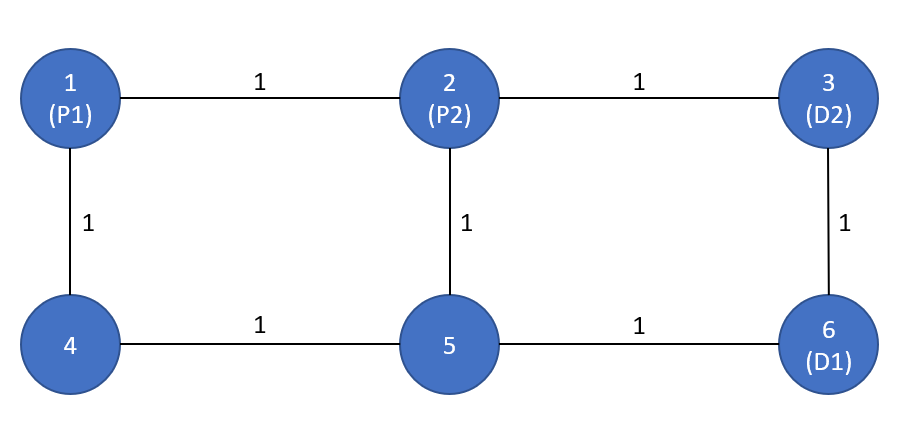
\includegraphics[width=1.0\textwidth]{resources/graph_init.png}
  \caption{Contoh tampilan antarmuka dari program}
\end{figure}

Pada umumnya kedua pesanan tersebut dilayani secara terpisah, contohnya pesanan satu 
memiliki rute $1-4-5-6$ yang memiliki \textit{cost} sebesar $3$ dan pesanan dua memiliki 
rute $2-3$ dengan \textit{cost} sebesar $1$. Hal tersebut diilustrasikan pada Gambar I.2.

\begin{figure}[H]
  \centering
  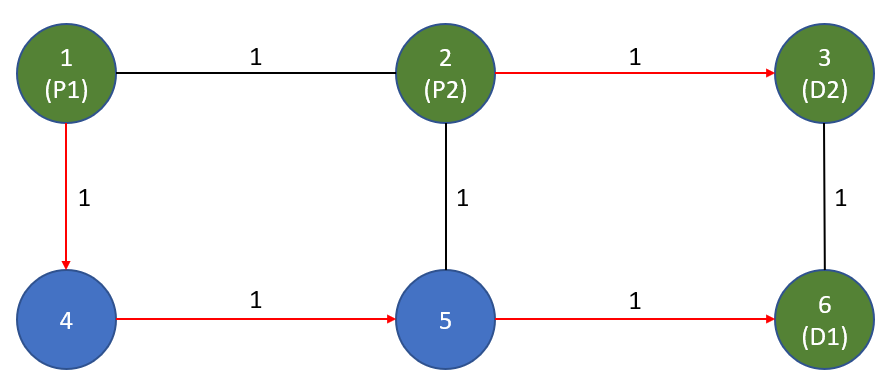
\includegraphics[width=1.0\textwidth]{resources/graph_routes.png}
  \caption{Graf yang memiliki rute 1-4-5-6 dan 2-3.}
\end{figure}

Namun, akan lebih efisien jika kedua pesanan tersebut dilakukan dalam sekali pengantaran 
seperti pada Gambar I.3, sehingga rute pengantarannya adalah $1-2-3-6$ dengan \textit{cost} 
sebesar $3$. Pada saat berada simpul 1, truk melakukan \textit{pickup}, lalu truk menuju 
simpul 2, dan melakukan \textit{pickup} barang pesanan ke-2. Setelah itu, truk menuju simpul 3 
dan menurunkan barang pesanan ke-2. Terakhir, truk menuju simpul 6  untuk melakukan 
\textit{drop off} pada barang pesanan ke-1.

\begin{figure}[H]
  \centering
  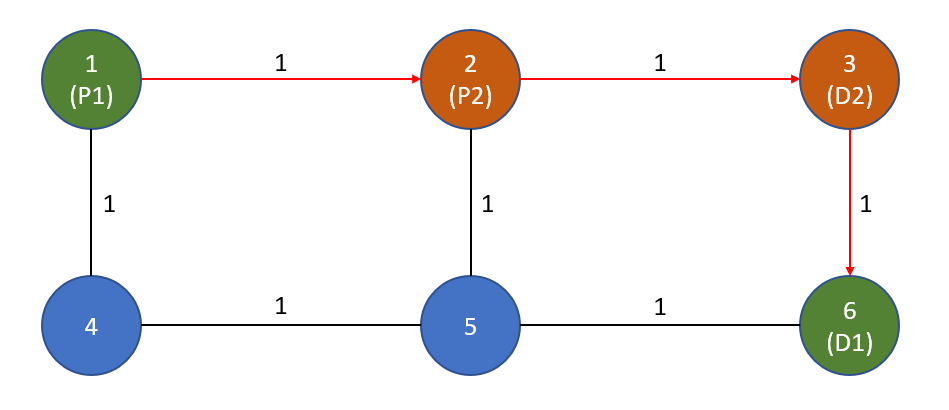
\includegraphics[width=1.0\textwidth]{resources/graph_optimal.png}
  \caption{Graf yang memiliki rute optimal 1-2-3-6.}
\end{figure}

\section{Rumusan Masalah}

Berdasarkan latar belakang pada subbab I.1, untuk menangani sebuah pesanan, dilakukan tepat 
sekali \textit{pickup} dan \textit{drop off}, namun telah ditunjukkan juga bahwa cara tersebut 
tidak selalu efisien dalam menangani banyak pesanan. 
Dari uraian tersebut, dapat dibentuk rumusan masalah sebagai berikut.

\begin{enumerate}
  % \item Bagaimana algoritma yang efisien untuk menentukan rute terbaik agar satu atau lebih pesanan dapat diselesaikan dalam sebuah rute pengantaran dengan sumber daya yang terbatas.
  % \item Apa indikator pengukuran suatu rute pengantaran, sehingga dapat dibandingkan dengan rute pengantaran lainnya?
  \item Bagaimana cara untuk menentukan rute pengantaran yang efisien sehingga dapat menyelesaikan satu atau lebih pengantaran?
\end{enumerate}

\section{Tujuan}

Berikut adalah tujuan yang ingin dicapai dalam penulisan tugas akhir ini:

\begin{enumerate}
  % \item Mengetahui indikator yang mengukur suatu rute pengantaran.
  \item Algoritma untuk menentukan rute terbaik agar satu atau lebih pesanan dapat diselesaikan dalam sebuah rute pengantaran dengan sumber daya yang terbatas.
\end{enumerate}

\section{Batasan Masalah}

Berikut adalah batasan-batasan masalah yang perlu diperhatikan:

\begin{enumerate}
  % \item Truk memiliki kapasitas maksimal, yang merupakan bilangan bulat positif.
  % \item Tiap pesanan memiliki cost bernilai bilangan bulat positif yang akan memakan kapasitas truk.
  % \item Penyimpanan truk bersifat LIFO atau last in first out.
  \item Selalu ada rute yang valid untuk setiap pesanan.
  \item Truk dapat melakukan \textit{drop off} suatu barang hanya setelah melakukan \textit{pickup}.
  % \item Truk dapat melakukan pengambilan barang dan pengiriman kapan saja.
  \item Daftar pickup dan \textit{drop off} sudah terdefinisi sebelum ditentukan rute truk.
\end{enumerate}

\section{Metodologi}

Berikut ini adalah tahapan dalam pengerjaan tugas akhir.

\begin{enumerate}
  \item Melakukan analisis terhadap permasalahan.\\
  Setelah mendapatkan definisi dari permasalahan, dilakukan analisis terhadap permasalahan, seperti masukan dan keluaran serta lingkup dan batasan permasalahan dan juga mempelajari algoritma shortest path untuk graf tak berarah.
  \item Mendesain algoritma.\\
  Pada tahap ini, dilakukan desain algoritma yang dapat menyelesaikan permasalahan dan memenuhi batasan-batasan masalah.
  \item Melakukan analisis dan pengujian algoritma.\\
  Terakhir, dilakukan analisis berupa kompleksitas algoritma, kebenaran algoritma, dan pengujian terhadap algoritma.
\end{enumerate}

\section{Jadwal Pelaksanaan Tugas Akhir}

Berikut adalah jadwal pengerjaan tugas akhir.

\begin{figure}[H]
  \centering
  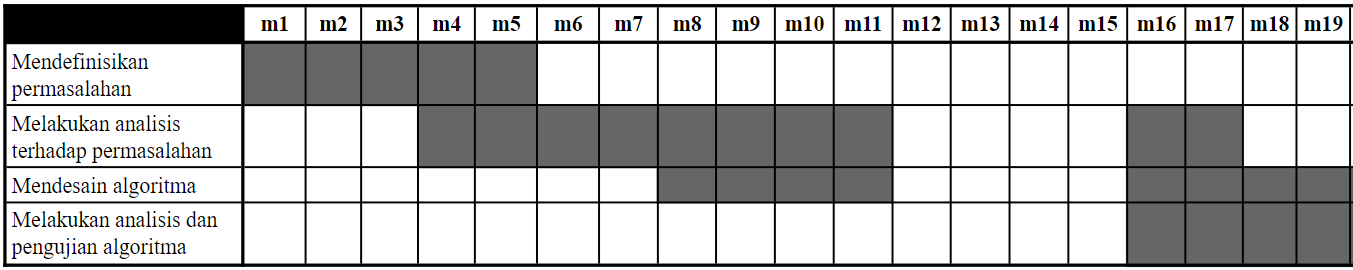
\includegraphics[width=1.0\textwidth]{resources/jadwal1.png}
  \caption{Jadwal pengerjaan tugas akhir bagian 1.}
\end{figure}

\begin{figure}[H]
  \centering
  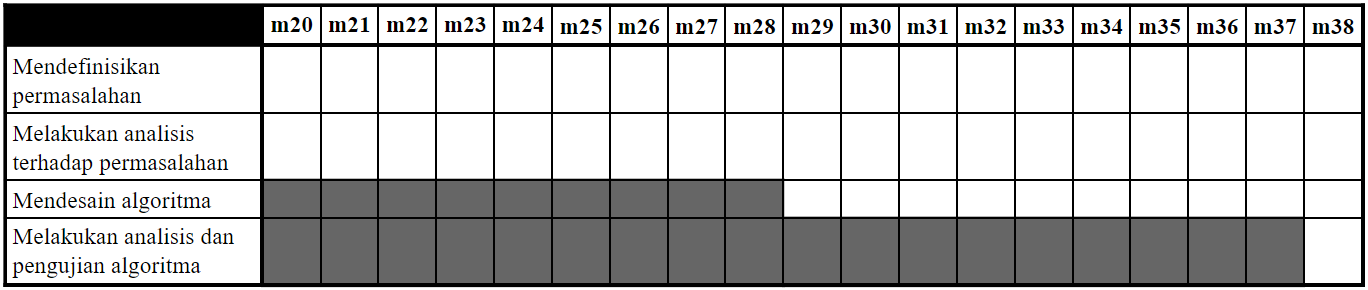
\includegraphics[width=1.0\textwidth]{resources/jadwal2.png}
  \caption{Jadwal pengerjaan tugas akhir bagian 2.}
\end{figure}

Keterangan:
\begin{itemize}
  \item m1: 30 September 2019 - 6 Oktober 2019
  \item m2: 7 Oktober 2019 - 13 Oktober 2019
  \item m3: 14 Oktober 2019 - 20 Oktober 2019
  \item m4: 21 Oktober 2019 - 20 Oktober 2019
  \item m5: 28 Oktober 2019 - 3 November 2019
  \item m6: 4 November 2019 - 10 November 2019
  \item m7: 11 November 2019 - 17 November 2019
  \item m8: 18 November 2019 - 24 November 2019
  \item m9: 25 November 2019 - 1 Desember 2019
  \item m10: 2 Desember 2019 - 8 Desember 2019
  \item m11: 9 Desember 2019 - 15 Desember 2019
  \item m12: 16 Desember 2019 - 22 Desember 2019
  \item m13: 23 Desember 2019 - 29 Desember 2019
  \item m14: 30 Desember 2019 - 5 Januari 2020
  \item m15: 6 Januari 2020 - 12 Januari 2020
  \item m16: 13 Januari 2020 - 19 Januari 2020
  \item m17: 20 Januari 2020 - 26 Januari 2020
  \item m18: 27 Januari 2020 - 2 Februari 2020
  \item m19: 3 Februari 2020 - 9 Februari 2020
  \item m20: 10 Februari 2020 - 16 Februari 2020
  \item m21: 17 Februari 2020 - 23 Februari 2020
  \item m22: 24 Februari 2020 - 1 Maret 2020
  \item m23: 2 Maret 2020 - 8 Maret 2020
  \item m24: 9 Maret 2020 - 15 Maret 2020
  \item m25: 16 Maret 2020 - 22 Maret 2020
  \item m26: 23 Maret 2020 - 29 Maret 2020
  \item m27: 30 Maret 2020 - 5 April 2020
  \item m28: 6 April 2020 - 12 April 2020
  \item m29: 13 April 2020 - 19 April 2020
  \item m30: 20 April 2020 - 26 April 2020
  \item m31: 27 April 2020 - 3 Mei 2020
  \item m32: 4 Mei 2020 - 10 Mei 2020
  \item m33: 11 Mei 2020 - 17 Mei 2020
  \item m34: 18 Mei 2020 - 24 Mei 2020
  \item m35: 25 Mei 2020 - 31 Mei 2020
  \item m36: 1 Juni 2020 - 7 Juni 2020
  \item m37: 8 Juni 2020 - 14 Juni 2020
  \item m38: 15 Juni 2020 - 21 Juni 2020
\end{itemize}

    \chapter{Studi Literatur}

\section{Logistik}

Kegiatan logistik merupakan penyampaian atau pengiriman barang atau material dalam 
jumlah tertentu dan waktu yang tepat ke suatu lokasi tertentu dengan biaya seminimal 
mungkin. Dari proses logistik, material atau barang dapat sampai ke tempat produksi 
melalui saluran distribusi, sehingga mampu memberikan kegunaan yang baik. Logistik yang 
dikelola dengan tepat, baik secara kuantitas maupun kualitas, kuantitas, maupun waktu 
dan biaya, dapan menjadi aset utama organisasi, yaitu sebagai sumber pendapatan yang 
strategis dan berperan mendorong kegiatan ekonomi. Logistik berasal dari kata logis yang 
berarti rasional dan tikos yang berarti berfikir, sehingga logistik memiliki arti 
berfikir rasioal dalam menjalankan kegiatan. 

Menurut Donald Bowersox, Logistik merupakan proses pengelolaan yang strategis terhadap 
pemindahan dan penyimpanan barang dari \textit{suplier} kepada perusahaan dan 
pelanggan. Ciri utama dari kegiatan logistik adalah keterpaduan berbagai dimensi dan 
tuntutan terhadap pemindahan (\textit{movement}) dan penyimpanan (\textit{storage}) yang 
strategis.


\section{\textit{Stack}}

\textit{Stack} adalah suatu struktur data dinamis yang mengikuti aturan \textit{LIFO} 
(\textit{Last In, First Out}) dalam melakukan operasinya. Terdapat tiga operasi pada 
struktur data ini, yaitu \textit{top}, \textit{push} (\textit{insert}), dan \textit{pop} 
(\textit{delete}). Operasi \textit{top} mendapatkan \textit{index} atau posisi dari 
elemen terakhir yang ditambahkan, \textit{push} menambahkan elemen ke \textit{stack}, 
dan \textit{pop} menghapus elemen yang paling terakhir ditambahkan.

Misalkan elemen pada \textit{stack} tersusun atas $S[1, 2, ..., S.top]$, dimana $S[1]$ 
merupakan elemen yang berada pada \textit{bottom} dari \textit{stack} dan $S[S.top]$ 
adalah elemen teratas dari \textit{stack}. \textit{Stack} kosong ketika $S.top$ bernilai 
0. \textit{Pseudocode} dari operasi struktur data \textit{stack} adalah sebagai berikut.

\medskip
\lstinputlisting[style=customc]{codes/stack-empty.txt}
\medskip
\lstinputlisting[style=customc]{codes/stack-push.txt}
\medskip
\lstinputlisting[style=customc]{codes/stack-pop.txt}

\section{Graf}

Graf adalah struktur diskrit yang terdiri atas simpul dan sisi yang menghubungkan 
simpul-simpul tersebut. Graf $G$ dapat didefinisikan sebagai sebuah \textit{tuple} yang 
terdiri atas himpunan simpul $V(G)$, himpunan sisi $E(G)$, dan himpunan relasi yang 
menghubungkan antara tepat dua buah simpul dan tepat sebuah sisi. Titik ujung dari suatu 
sisi adalah dua buah simpul yang terhubung pada sisi tersebut. Cincin adalah sisi yang 
kedua simpul di ujungnya sama. Graf disebut sederhana jika tidak memiliki lebih dari 
satu sisi yang menghubungkan pasangan simpul berbeda yang sama dan tidak memiliki cincin. 
Graf berbobot adalah graf yang setiap sisi-sisinya memiliki bobot atau nilai.

Graf berarah adalah graf yang setiap sisi-sisinya dikaitkan dengan suatu arah. Sisi pada 
graf berarah dapat di representasikan dengan $e (u, v)$ yang mana sisi $e$ memiliki arah 
dan menghubungkan simpul $u$ dan simpul $v$ serta arah dari sisi tersebut adalah dari $u$ 
ke $v$. Dengan menggunakan sisi tersebut dari simpul $u$ dapat menuju simpul $v$, namun 
tidak sebaliknya. Graf yang setiap sisi-sisinya tidak memiliki arah disebut dengan graf 
tak berarah.

\section{Jalur}

Jalur dapat didefinisikan sebagai berikut. Misalkan $n$ merupakan bilangan bulat tak 
negatif dan $G$ merupakan suatu graf. Sebuah jalur dengan panjang $n$ dari simpul $u$ 
ke simpul $v$ adalah rangkaian yang tersusun atas $n$ buah sisi 
$e_{1}, e_{2}, ..., e_{n}$ yang mana untuk setiap $1 \leq i \leq n$, $e_{i}$ merupakan 
sisi di $G$ dan sisi $e_{i}$ menghubungkan simpul $v_{i-1}$ dengan simpul $v_{i}$ serta 
$x_{0} = u$ dan $x_{n} = v$. Singkatnya, jalur adalah rangkaian dari sisi-sisi yang 
dimulai dari suatu simpul dan bergerak dari simpul ke simpul yang terhubung dengan sisi 
pada graf. Suatu jalur yang dimulai dan diakhiri pada simpul yang sama disebut dengan 
sirkuit, yang mana $v_{0} = v_{n}$ dan minimal melewati sebuah sisi. Suatu jalur disebut 
sederhana jika sisi yang dilewati jalur tersebut tidak berulang.

Panjang sebuah jalur pada graf tak berbobot adalah jumlah dari sisi-sisi yang dilewati. 
Panjang dari jalur pada graf berbobot adalah jumlah bobot dari sisi yang dilewati.

\section{Menjelajahi Graf}

Menjelajahi graf adalah suatu proses untuk mengunjungi setiap simpul pada suatu graf. 
Berikut adalah algoritma-algoritma yang sering digunakan untuk menjelajahi graf.

  \subsection{\textit{Breadth-First Search}}
  Misalkan terdapat sebuah graf $G = (V, E)$ dan sebuah simpul awal $s$. Algoritma ini 
  melakukan penjelajahan secara melebar pada setiap \textit{level}. Pertama-tama 
  algoritma ini mengunjungi simpul awal $s$ sebagai simpul pada \textit{level} ke-0. 
  Lalu, setiap simpul yang yang bersebelahan dengan simpul $s$ akan menjadi 
  simpul-simpul pada \textit{level} ke-1 dan algoritma ini akan mengunjungi 
  simpul-simpul tersebut. Setelah itu, semua simpul yang bersebelahan dengan 
  simpul-simpul pada \textit{level} ke-1 dan belum pernah dikunjungi, akan dijadikan 
  simpul-simpul pada \textit{level} ke-2 dan akan dikunjungi. Hal ini dilakukan terus 
  menerus hingga semua simpul yang dapat dikunjungi dari $s$  telah dikunjungi. 
  Algoritma ini menggunakan struktur data \textit{queue} dalam melakukan penjelajahan. 
  Berikut adalah \textit{pseudocde} dari algoritma \textit{breadth-first search}.

  \medskip
  \lstinputlisting[style=customc, mathescape=true]{codes/bfs.txt}

  \subsection{\textit{Depth-First Search}}
  Misalkan terdapat sebuah graf $G = (V, E)$, sebuah simpul awal $s$, dan 
  $s_{0}, s_{1}, ..., s_{k}$ sebagai simpul-simpul yang bersebelahan dengan $s$. 
  Algoritma \textit{depth-first search} menjelajahi graf dengan mengunjungi anak dari 
  suatu simpul terlebih dahulu. Pertama-tama algoritma ini mengunjungi simpul $s$. 
  Lalu, memilih salah satu simpul, misalkan $s_{0}$, yang bersebelahan dengan $s$ dan 
  belum dikunjungi sebagai simpul awal. Setelah tidak ada lagi simpul yang dapat 
  dikujungi dari $s_{0}$, algoritma ini memilih simpul lain, misalkan $s_{1}$, yang 
  bersebelahan dengan $s$ dan belum dikunjungi. Hal ini dilakukan terus-menerus hingga 
  semua simpul yang dapat dikunjungi dari $s$ telah dikunjungi.

  \medskip
  \lstinputlisting[style=customc, mathescape=true]{codes/dfs.txt}

\section{Persoalan Jalur Terpendek}

Jalur terpendek dari simpul $u$ ke simpul $v$ adalah jalur yang dimulai dari simpul $u$ 
dan diakhiri pada simpul $v$ yang memiliki panjang minimum. Persoalan jalur terpendek 
dapat dibagi menjadi 4 variasi, yaitu persoalan jalur terpendek dari simpul $u$ ke 
simpul $v$, persoalan jalur terpendek yang dimulai dari suatu simpul, jalur terpendek 
untuk setiap pasangan simpul pada graf, dan jalur terpendek yang berakhir pada suatu 
simpul. Jalur terpendek memiliki suatu sifat, yaitu sub-jalur dari suatu jalur terpendek 
adalah sebuah jalur terpendek. Agar dapat menyimpan jalur terpendek, akan digunakan 
$P(V)$ yang mana untuk tiap $p_{i}$ pada $P(V)$ merupakan pendahulu pada jalur terpendek 
yang diakhiri di simpul $i$, sehingga untuk mendapatkan jalur terpendek yang diakhiri 
pada simpul ke $u$, dapat dilakukan dengan mencari pendahulu-pendahulu dari simpul 
tersebut.

\medskip
\lstinputlisting[style=customc]{codes/get-path.txt}

Salah satu permasalahan yang dihadapi dalam melakukan pencarian jalur terpendek adalah 
ketika terdapat \textit{negative cycle} yang dapat dicapai dari simpul awal. 
\textit{Negative cycle} adalah sirkuit yang memiliki panjang yang negatif. Ketika 
terdapat sirkuit yang dapat dicapai dari $s$, maka terdapat tak hingga jalur yang dapat 
dibentuk. Jika sirkuit tersebut memiliki panjang yang negatif, dapat dibuktikan bahwa 
tidak ada jalur terpendek yang dimulai dari simpul $s$.

Pada suatu jalur terpendek, mustahil terdapat sirkuit dengan  panjang positif. Misalkan 
$p = [v_{0}, v_{1}, v_{2}, v_{3}, ..., v_{n}]$ adalah jalur terpendek, 
$c = [v_{i}, v_{i+1}, ..., v_{j-1}, v_{j}]$ adalah sirkuit dengan panjang positif yang 
terdapat pada $p$, $L(x)$ adalah panjang dari jalur $x$, dan 
$p’ = [v_{0}, v_{1}, ..., v_{i}, v_{j+1}, …, v_{n}]$ adalah jalur $p$ tanpa sirkuit $c$. 
Jalur $p’$ memiliki panjang $L(p’)$ dan $L(p’) = L(p) - L(c) < L(p)$. Panjang jalur 
$p’$ lebih kecil dari pada panjang jalur $p$, sehingga $p$ tidak mungkin menjadi jalur 
terpendek.

Pada bahasan subbab dibawah ini, akan digunakan teknik relaxation. Teknik ini menyimpan 
$D(V)$ sebagai batas atas jarak terpendek dari simpul $s$, yang mana di adalah batas 
atas jarak terpendek dari simpul $s$ ke simpul $i$. Proses relaxing pada sisi $(u, v)$ 
terdiri atas mengecek apakah estimasi jalur terpendek menuju $v$ dapat di perkecil dan 
mengubah estimasi panjang jalur terpendek. Selain itu, juga akan dipakai fungsi 
\textit{init-single-source} yang merupakan fungsi untuk melakukan inisialisasi pada 
nilai $P(V)$ dan $D(V)$ serta fungsi relax yang akan menerapkan teknik 
\textit{relaxation} pada sisi $(u,v)$.

\medskip
\lstinputlisting[style=customc, mathescape=true]{codes/init-single-source.txt}

\medskip
\lstinputlisting[style=customc]{codes/relax.txt}

Dalam menentukan jalur terpendek maupun panjang jalur terpendek, terdapat beberapa 
algoritma-algoritma seperti berikut.

  \subsection{Algoritma Bellman-Ford}
  Algoritma Bellman-Ford menyelesaikan persoalan jalur terpendek yang dimulai dari 
  suatu simpul dengan menggunakan pendekatan pemrograman dinamis. Algoritma 
  Bellman-Ford juga dapat menangani kasus \textit{negative cycle}. Diberikan graf 
  $G = (V, E, W)$ dengan simpul awal jalur adalah $s$, algoritma Bellman-Ford 
  mengembalikan \textit{boolean true} jika tidak terdapat \textit{negative cycle} 
  dalam jalur terpendek dan algoritma ini akan menghasilkan jalur terpendek yang 
  berasal dari simpul $s$. Algoritma ini melakukan \textit{}{relaxation} secara 
  terus-menerus terhadap sisi-sisi pada graf, sehingga memperkecil nilai estimasi 
  panjang jalur terpendek $D(V)$ hingga mencapai panjang jalur terpendek yang 
  sebenarnya. Berikut adalah \textit{pseudocode} dari algoritma Bellman-Ford.

  \medskip
  \lstinputlisting[style=customc]{codes/bellman-ford.txt}

  Kompleksitas waktu dari algoritma Bellman-Ford adalah $O(VE)$. Algoritma Bellman-Ford 
  dapat digunakan untuk mencari jalur terpendek setiap pasangan simpul pada graf, 
  dengan memanggil fungsi Bellman-Ford untuk setiap simpul pada graf.  Dalam hal 
  tersebut kompleksitas waktunya adalah $O(VVE)$.

  \subsection{Algoritma Dijkstra}
  Algoritma Dijkstra menyelesaikan persoalan jalur terpendek yang dimulai dari suatu 
  simpul melalui pendekatan greedy. Diberikan graf berarah dan berbobot 
  $G = (V, E, W)$, yang mana setiap sisi memiliki bobot yang merupakan bilangan tak 
  negatif dan simpul $s$ yang merupakan simpul awal. Algoritma Dijkstra menyimpan 
  himpunan simpul $U$ yang mana untuk tiap simpul pada $U$, sudah ditentukan jalur 
  terpendek dari $s$. Algoritma ini berulang kali mengambil sebuah simpul $a$ pada 
  $V - U$ yang mempunyai jarak terpendek yang telah diestimasi lalu menambahkan $a$ 
  ke himpunan $U$. Setelah itu, melakukan relaxation kepada semua sisi yang keluar 
  dari $a$. Berikut adalah \textit{pseudocode} dari algoritma Dijkstra.

  \medskip
  \lstinputlisting[style=customc, mathescape=true]{codes/dijkstra.txt}

  Kompleksitas waktu dari algoritma Dijkstra adalah $O(V^{2} + E)$. Ketika menggunakan 
  struktur data seperti \textit{self-balancing binary search tree} atau \textit{heap} 
  pada $U$ dan $V$, kompleksitas waktu dari algoritma ini dapat mencapai 
  $O((V + E) * \log V)$.

  Algoritma Dijkstra dapat digunakan untuk mencari jalur terpendek setiap pasangan 
  simpul pada graf, dengan memanggil fungsi Dijkstra untuk setiap simpul pada graf. 
  Dalam hal tersebut kompleksitas waktunya adalah $O(V*(V + E)* \log V)$.

  \subsection{Algoritma Floyd-Warshall}
  Algoritma Floyd-Warshall menggunakan pendekatan pemrograman dinamis dalam menemukan 
  jalur terpendek untuk setiap pasangan simpul pada graf berarah dan berbobot 
  $G = (V, E, W)$. Dalam menentukan jalur terpendek $(u,v)$, algoritma ini 
  memperhatikan simpul intermediate, yaitu pada jalur 
  $p = [v_{1}, v_{2}, v_{3}, ..., v_{n}]$, simpul intermediate adalah simpul yang 
  bukan $v_{1}$ ataupun $v_{n}$. Algoritma ini bergantung pada observasi berikut. 
  Misalkan $V = {1, 2, 3, ..., n}$ adalah simpul-simpul pada graf, $R = {1, 2, ..., k}$ 
  adalah himpunan bagian dari $V$, untuk jalur terpendek dari setiap pasangan $(i, j)$ 
  pada $V$ yang memiliki simpul intermediate dari $R$, dan $p$ adalah jalur terpendek 
  dari pasangan-pasangan simpul tersebut. Hubungan dari $k$ dengan $p$ adalah sebagai 
  berikut.

  \begin{enumerate}
    \item Jika $k$ bukan simpul intermediate dari $p$, maka simpul-simpul intermediate dari $p$ adalah $R’ = {1, 2, ..., k-1}$.
    \item Jika $k$ adalah simpul intermediate dari $p$, jalur terpendek $p$ dapat didekomposisi menjadi jalur terpendek $p^{(1)}$ dari $i$ ke $k$ 
    dan jalur terpendek $p^{(2)}$ dari $k$ ke $j$. Simpul-simpul intermediate dari $p^{(1)}$ dan $p^{(2)}$ adalah dari $R’ = {1, 2, ..., k-1}$.
  \end{enumerate}

  Ketika $k$ bernilai 0, tidak ada simpul \textit{intermediate} pada $p$. Dari 
  observasi di atas, dapat dibuat relasi rekurens untuk menghitung jalur terpendek 
  dari $p$, yaitu
  \begin{equation}
    d_{i,j}^{(k)} =
    \begin{cases}
      d_{i,j}^{(0)}, & \text{if } k = 0\\
      min(d_{i,j}^{(k)}, d_{i,k}^{(k-1)} + d_{k,j}^{(k-1)}), & \text{otherwise}.
    \end{cases}
  \end{equation}
  dimana $d_{i,j}^{(n)}$ adalah panjang dari jalur terpendek dari i ke j. Dari relasi rekurens diatas, dapat dibuat pseudocode dari algoritma Floyd-Warshall sebagai berikut.

  \medskip
  \lstinputlisting[style=customc, mathescape=true]{codes/floyd-warshall.txt}

  Kompleksitas waktu dari algoritma Floyd-Warshall adalah $O(V^{3})$.

    \chapter{Definisi Masalah Dan Rancangan Algoritma Pencarian Rute Pengantaran}

\section{Definisi Formal Permasalahan}

Diberikan suatu graf berarah dan berbobot $G$ yang memiliki himpunan simpul $V(G)$, himpunan sisi
$E(G)$, dan himpunan bobot $W(E(G))$ yang merupakan bobot pada tiap sisi di $G$. Diberikan juga $n$
buah pesanan $P$ yang tiap pesanan $p_{i}$ untuk $1 \leq i \leq n$ berupa \textit{tuple} $(a_{i},
b_{i}, c_{i})$, dimana $a_{i}$ dan $b_{i}$ merupakan simpul pada graf $G$, $a_{i}$ adalah simpul
tempat pengambilan barang pesanan ke-$i$, $b_{i}$ adalah simpul tempat penurunan barang pesanan
ke-$i$, dan $c_{i}$ adalah ukuran barang yang akan diantar pada pesanan ke-$i$. Terdapat $m$ truk
yang dapat digunakan untuk melakukan pengantaran. Penyimpanan truk memiliki sifat yang sama dengan
struktur data \textit{stack}. Setiap truk memiliki kapasitas maksimum penyimpanan yang sama berupa
bilangan bulat positif yang dilambangkan dengan $C$ .

Dari info yang diberikan, masalah yang ingin diselesaikan adalah sebuah jalur yang akan 
dilewati oleh setiap truk, yang memenuhi syarat berikut:
\begin{enumerate}
  \item Setiap bobot dari sisi pada graf $G$ adalah bilangan bulat positif.
  \item Setiap pesanan memiliki \textit{cost} $c_{i}$ bernilai bilangan bulat positif yang akan
  memakan kapasitas truk.
  \item Penyimpanan truk bersifat LIFO atau \textit{last in, first out}.
  \item Penurunan barang pada pesanan $p_{i}$ hanya dapat dilakukan setelah barang pada pesanan
  $p_{i}$ diambil.
  \item Barang yang hanya dapat diturunkan hanya jika berada pada atas penyimpanan.
  \item Jumlah ukuran barang yang terdapat pada penyimpanan suatu truk tidak melebihi kapasitasnya.
\end{enumerate}

Indikator pengukuran dari suatu rute adalah jumlah bobot dari sisi-sisi yang dilalui oleh semua truk
yang akan dilambangkan dengan $T$. Bobot disini berupa jumlah jarak tempuh yang dilalui oleh semua
truk pada rute yang ditentukan. Pencarian rute ini memiliki objektif, yaitu meminimalkan nilai
dari $T$ dan meminimalkan jumlah truk yang digunakan.

\section{Rancangan Algoritma 1}

Dalam menyelesaikan persoalan tersebut, hal yang perlu diperhatikan hanyalah simpul-simpul
\textit{pickup} dan \textit{drop off} pesanan, sehingga graf $G$ dapat direduksi menjadi graf $G’$,
yang mana simpul-simpul pada graf $G’$ memuat simpul-simpul tempat \textit{pickup} barang dan
\textit{drop off} barang. Sisi-sisi dari graf $G’$ adalah jalur terpendek antara tiap dua simpul
pada graf $G'$. Perhitungan jalur terpendek ini menggunakan sisi-sisi yang berasal dari graf $G$.

Selanjutnya, hal yang dicari adalah suatu jalur yang memiliki panjang minimal dan menggunakan truk
sesedikit mungkin yang memenuhi syarat-syarat dari permasalahan diatas. Pencarian rute optimal akan
dilakukan dengan menggunakan \textit{backtracking} yang dimulai dari setiap simpul \textit{pickup}.
Algoritma ini menyimpan barang yang berada dalam truk pada struktur data \textit{stack}. Misalkan
$S$ adalah simpul-simpul tempat \textit{pickup}. Dalam melakukan \textit{backtracking}, jika
terdapat barang pesanan dalam truk, algoritma ini akan mencoba menelusuri kemungkinan jalur ketika
melakukan \textit{drop off} barang terakhir pada \textit{stack}. Ketika masih terdapat simpul
\textit{pickup} pada $P$ dan kapasitas dari truk masih mencukupi, algoritma ini juga akan mencoba
kemungkinan dari setiap simpul pada $P$. Jika mengambil simpul dari $P$, maka simpul \textit{drop
off}-nya akan ditambahkan ke \textit{stack}. Selain itu, Ketika masih truk yang tersisa, algoritma
ini juga akan menyusuri kemungkinan dengan menggunakan truk lain. Terakhir, ketika tidak ada lagi
pesanan pada $P$ dan \textit{stack} kosong, maka algoritma ini akan membandingkan mana jalur yang
paling baik dengan jalur yang sudah dihitung sebelumnya. Berikut adalah \textit{pseodocode} dari
rancangan algoritma 1.

\medskip
\lstinputlisting[style=customc, mathescape=true]{codes/ra1.txt}

\section{Rancangan Algoritma 2}

Dari rancangan algoritma 1, dapat diterapkan metode \textit{dynamic programming} dengan menyimpan
\textit{state} atau keadaan dari pesanan-pesanan yang belum diambil, sudah diambil, dan sudah
diantar dimisalkan dengan $item_state$. Keadaan lain yang perlu disimpan adalah barang-barang yang
berada di dalam \textit{stack} yang dimisalkan dengan $storage_state$ serta jumlah truk yang tersisa
dimisalkan dengan $m_state$. Untuk setiap $item_state$, $storage_state$, dan $m_state$, disimpan
jarak minimal yang dapat ditempuh untuk mengantarkan semua barang. Hal ini lebih efisien dalam
jumlah perhitungan yang perlu dilakukan karena setiap keadaan hanya dihitung maksimal satu kali.

% \section{Rancangan Algoritma 3}


    % \input{chapters/chapter-4}
    % \input{chapters/chapter-5}
    %----------------------------------------------------------------%

    % Daftar pustaka
    \nocite{*}
    \printbibliography[title=Daftar Pustaka]
    \addcontentsline{toc}{chapter}{Daftar Pustaka}

    % Index
    % \appendix

    % \addcontentsline{toc}{part}{Lampiran}
    % \part*{Lampiran}

    % \input{chapters/appendix-1}
    % \input{chapters/appendix-2}

\end{document}
